\chapter{Bruit 5G}

Lorsqu'un appareil émet sur le spectre de la 5G, il devient particulièrement sensible aux interférences électromagnétiques voire figure \ref{fig:bruit-5g}. Cela peut fausser les mesures réalisées à proximité, car les signaux émis peuvent perturber les instruments de mesure. Il est donc essentiel d'éloigner les appareils émettant sur ces fréquences afin de garantir la fiabilité et la précision des résultats obtenus.
\begin{figure}[H]
    \centering
    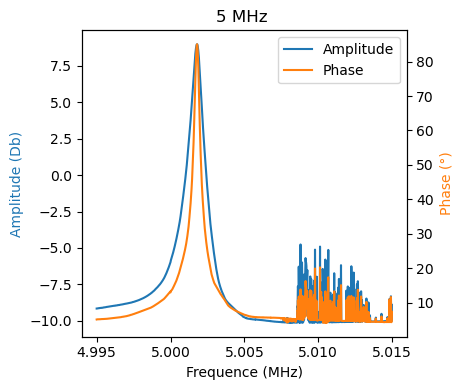
\includegraphics[width=0.8\textwidth]{assets/figures/bruit5G.png}
    \caption{Illustration du bruit 5G}
    \label{fig:bruit-5g}
\end{figure}

\chapter{Choix harmoniques}
\label{chap:choix_harmoniques}
Les mesure de frequance et d'amplitude on été faite sur trois harmoniques du quartz, la 1ère, la 3ème et la 5ème.
La 3 ème harmonique a été choisi pour les resulat lors du chapitre \ref{chap:application_experimentale} car elle presente le moin de bruit, la 1ère et la 5ème harmonique sont trop bruitées pour être utilisables.
voici un exemple  de mesure avec de l'eau avec les trois harmoniques, on peut voir que la 3ème est la plus stable.

\begin{figure}[H]
    \centering
    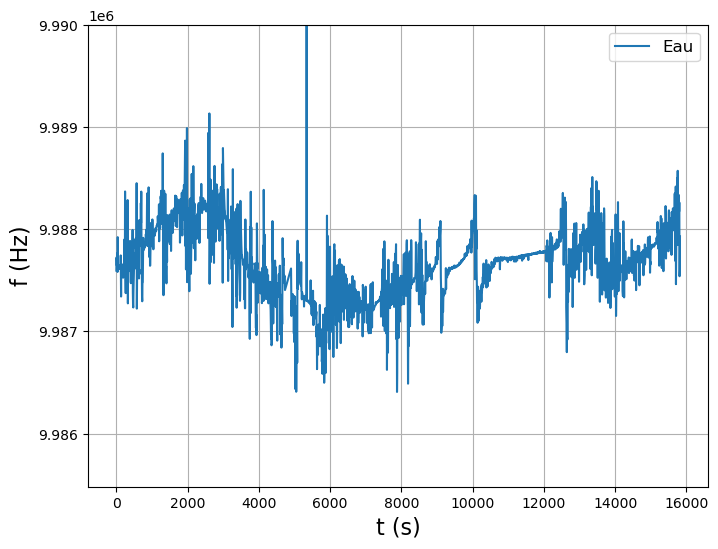
\includegraphics[width=0.8\textwidth]{assets/figures/annex10MHzFrequ.png}
    \caption{Mesure de la 1ère harmonique à 10Mhz avec de l'eau}
    \label{fig:choix_harmonique10MHz}
\end{figure}

\begin{figure}[H]
    \centering
    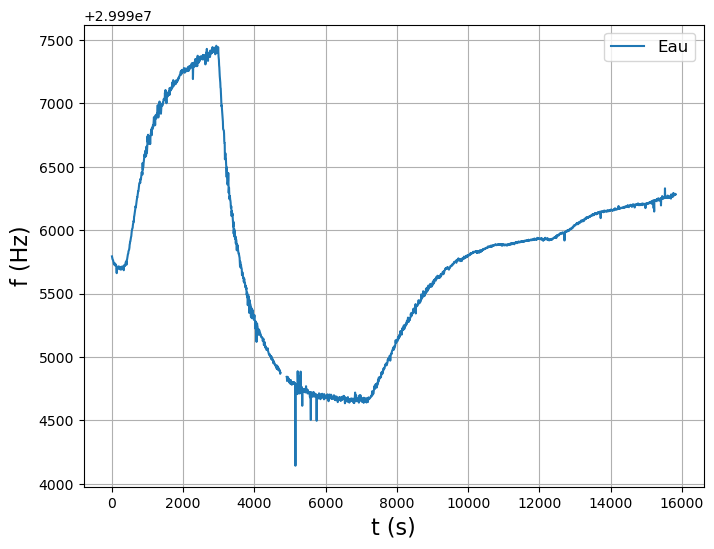
\includegraphics[width=0.8\textwidth]{assets/figures/annex30MHzFrequ.png}
    \caption{Mesure de la 3ème harmonique à 30Mhz avec de l'eau}
    \label{fig:choix_harmonique30MHz}
\end{figure}

\begin{figure}[H]
    \centering
    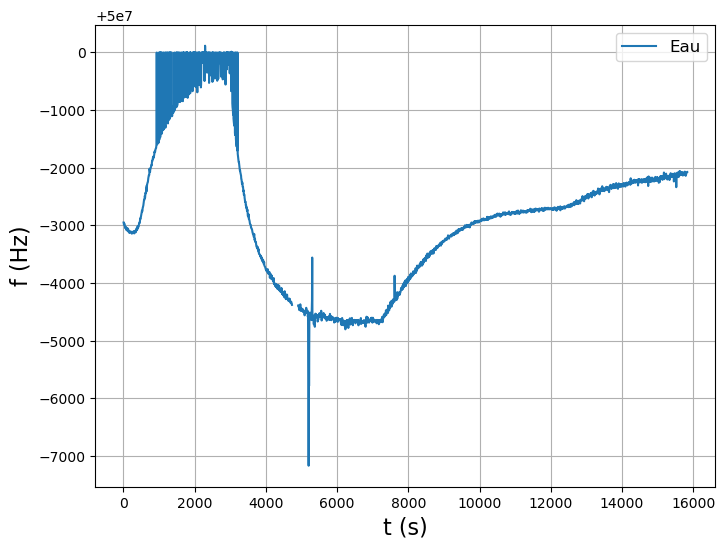
\includegraphics[width=0.8\textwidth]{assets/figures/annex50MHzFrequ.png}
    \caption{Mesure de la 5ème harmonique à 50Mhz avec de l'eau}
    \label{fig:choix_harmonique50MHz}
\end{figure}
\chapter{Manuel d'utilisation QCMApp}
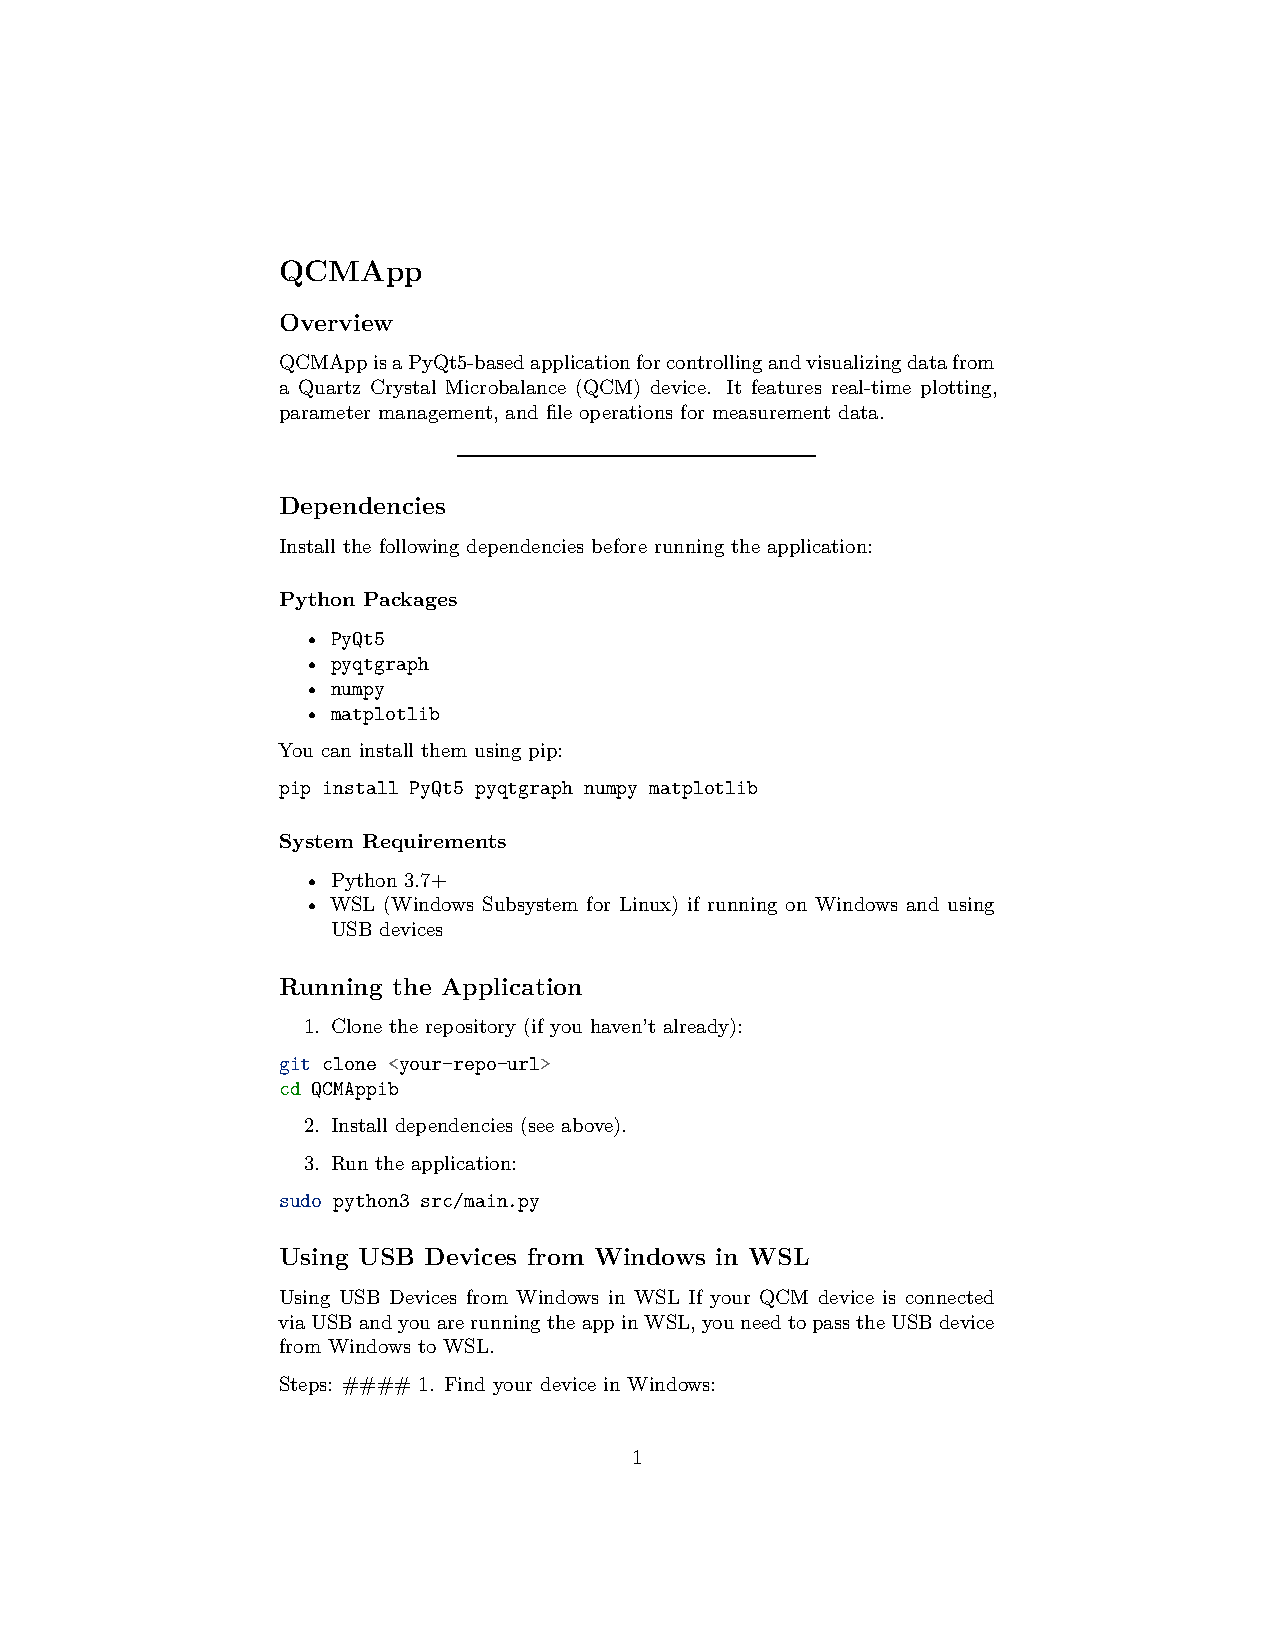
\includepdf[pages=-]{assets/readme.pdf}